\documentclass[a4paper,10pt]{article} 

\usepackage[utf8]{inputenc} 
%\usepackage[T1]{fontenc}

\usepackage{textcomp}           % Extra Symbole (Grad Celsius etc.)
\usepackage{amssymb,amsmath}    % Schöne Formeln (AMS = American Mathematical Society)
\usepackage{graphicx}           % Bilder und Seitenränder
\usepackage{subcaption}			% captions for subfigures
\usepackage{booktabs}           % Schönere Tabellen
\usepackage{colortbl}           % Farbige Tabellen

%\usepackage{tcolorbox}			% schöne bunte Boxen
\usepackage{mathtools}			% \mathclap für ordentliche \underbrace-			environments
\usepackage{geometry}			% Pagelayout mit \newgeometry, \restoregeometry
\usepackage{float}
\usepackage{wrapfig}
\usepackage{enumitem}
\usepackage{float}
\usepackage{braket}
\usepackage{caption}
\usepackage{gensymb}
\usepackage[version=4]{mhchem}
\input{insbox.tex}
%\usepackage{pst-optexp}
%\usepackage{auto-pst-pdf}

\graphicspath{{./img/}}


\bibliographystyle{unsrtnat}

\renewcommand{\k}{\mathbf{k}}
\begin{document}
\begin{titlepage}
 \begin{center}
	\Large{Advanced laboratory class 2}
	\end{center}
	\begin{center}
	 \LARGE{\textbf{FP2 - Diode Laser With Optical Feedback}}
	\end{center}
	
	\begin{center}
	
	\large Marco \textsc{Canteri} \\
	marco.canteri@student.uibk.ac.at
	\end{center}
	
	\begin{center}
	\vspace{1cm}
	Innsbruck, \today
	\vspace{2cm}
	\end{center}
	
	\begin{center}
	
\includegraphics[scale=0.4]{img/uibk} 
	\end{center}

\end{titlepage}
\begin{abstract}
In this experiment we first characterized a diode laser, then we studied the influence of optical feedback on the laser output. The feedback was provided by means of an external optical cavity which we built in the Littrow and Littman configuration. In both of these configurations we determined the laser wavelength and the lasing threshold. Finally we studied the laser tunability in the Littman configuration.
\end{abstract}
\section{Introduction}
A free running diode laser has a linewidth in the order of 10 MHz \cite{skriptum}, this is not enough to perform high-resolution spectroscopy for instance. Moreover, the output of a diode laser is often multimode \cite{tunablelaser}, which leads to possible mode hopping. The tunability is also limited, temperature and current do not provide a continuous and reliable tuning \cite{lasertunability}. Nevertheless, the performances of a diode laser can be enhanced with optical feedback: with this technique the linewidth can be narrowed down, and the wavelength can be tuned more precisely \cite{lasermodulation}. Optical feedback is provided by an external cavity which can be built in several ways. In this work we explored two different configurations, so called Littrow and Littman configuration. By analyzing the geometry of the configurations it was possible to determine the wavelength of the laser, and by tuning the input current, we were able to find the lasing threshold in the various configurations.
\section{Theory}
A diode laser is a semiconductor device used to create a laser beam. A diode laser has two main components, an active gain medium, and an optical resonator. The active region is a pn-junction, electron and holes from the two layers are injected into the depletion region. Here they recombine and emit photons by means of spontaneous emission. In the simplest case the optical resonator is a Fabry-Perot of length $L$ (typically hundreds of micrometers). Created photons that travel in the Fabry-Perot enhance the recombination effect of electrons and holes by stimulated emission. This leads to an amplification of the light inside the cavity, however inside the same cavity there are losses due to free-carrier absorption, scattering, and mirror losses \cite{tunablelaser}. Therefore, when the gain inside the cavity overcome the losses, stimulated emission dominates spontaneous emission and the laser is said to be lasing. If we consider a Fabry-Perot which has facets with power reflectivity $R_1$ and $R_2$, we can write the round trip gain $G$ inside the cavity as \cite{lasermodulation}
\begin{equation}G = \sqrt{R_1R_2}e^{(g-a)L}e^{-2i\beta L},\end{equation}
where $\beta$ is a phase constant, $g$ the gain, and $a$ the internal losses. The lasing threshold is when the round trip gain is unitary, so we have the condition
\begin{equation}g_{th} = a + \frac{1}{2L}\ln\left(\frac{1}{R_1 R_2}\right),\end{equation}
which is the lasing threshold. Above the lasing threshold the laser output increases of order of magnitude. To overcome the threshold the gain has to increase, which can be done by changing the injection current of the laser.\\
The output of the diode laser is a multimode spectrum, in fact the gain is frequency dependent, so several mode can be above the lasing threshold. The linewidth of the modes is given by the Schawlow–Townes formula \cite{linewidthformula}
\begin{equation}\Delta \nu = \frac{4\pi h\nu (\Delta\nu_c)^2}{P_{out}},\end{equation}
where $\nu$ is the frequency, $\Delta\nu_c$ is the resonator bandwidth, and $P_{out}$ is the output power of the laser. The linewidth can be narrowed down with optical feedback, and the bandwidth can be reduced, which minimize the possibility of mode hopping. Optical feedback is a technique which consist of sending a part of the output light back into the laser by means of external cavity. In figure \ref{setup} two possible configuration of external cavities are presented. The role of the feedback is to change the gain inside the laser and therefore excite a particular mode. From a mathematical point of view, it is possible to introduce an effective reflection coefficient \cite{feedback} instead of having the reflectivity $R_2$.

\section{Experiment setup}
\begin{figure}[H]
    \centering
    \begin{subfigure}[b]{0.36\textwidth}
        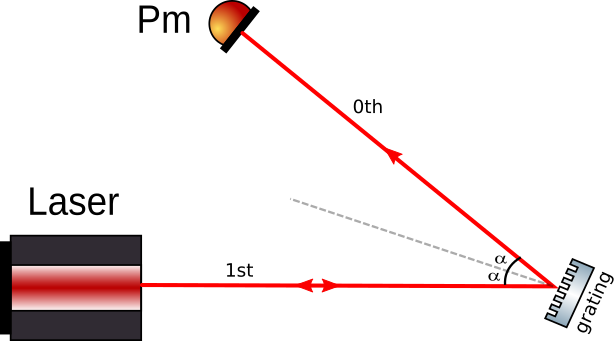
\includegraphics[width=\textwidth]{littrow}
        \caption{Littrow configuration}\label{littrow}
    \end{subfigure}
    \hfill
    \begin{subfigure}[b]{0.62\textwidth}
        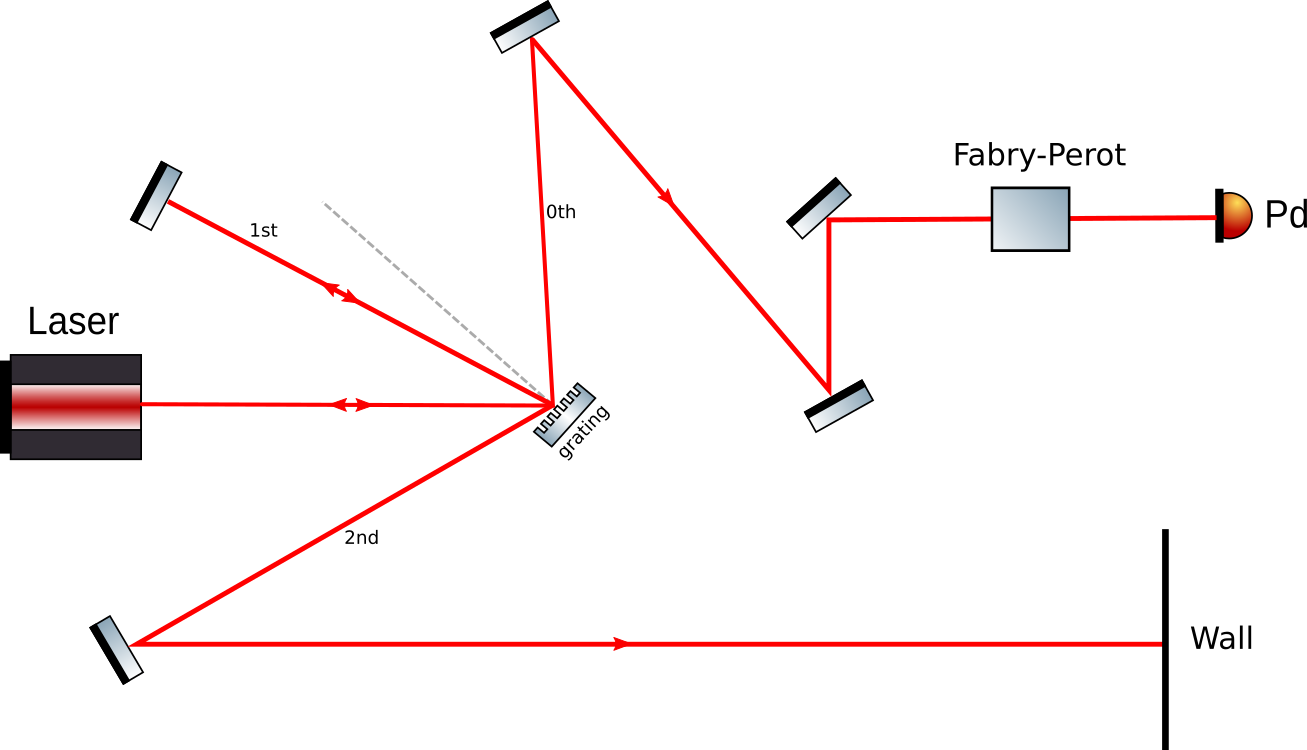
\includegraphics[width=\textwidth]{littman}
        \caption{Littman configuration}\label{littman}
    \end{subfigure}
\caption{Experiment setups. Pm is a powermeter, while Pd stands for photodiode. The numbers indicate the diffraction order of the beam, while the dashed gray line is the grating's normal}\label{setup}
\end{figure}
The experiment had two different setups, both are show in figure \ref{setup}. In the Littrow configuration the light source is a diode laser. The light is sent to a blazed grating with a line spacing of $d=$1200/mm. The incidence angle is chosen such that the first diffraction order is back reflected and sent into the laser to provide optical feedback. The zeroth order beam is measured with a powermeter.\\
The same laser diode and the same grating are used in the Littman configuration. The orientation of the grating is chosen such that the first order beam hits a mirror and is sent back to the grating and then into the laser in order to provide again optical feedback. The zeroth order beam is coupled into a Fabry-Perot with the help of three mirrors. The Fabry-Perot mirrors are controlled with a cylindrical piezoelectric crystal, which allows us to tune the length of the Fabry-Perot cavity with a function generator. After the Fabry-Perot, the light is  measured with a photodiode. Furthermore, the second order beam is sent to a piece of paper placed on the wall.

\section{Data analysis}
\subsection{Diode laser characterization}
\begin{figure}[H]
\centering
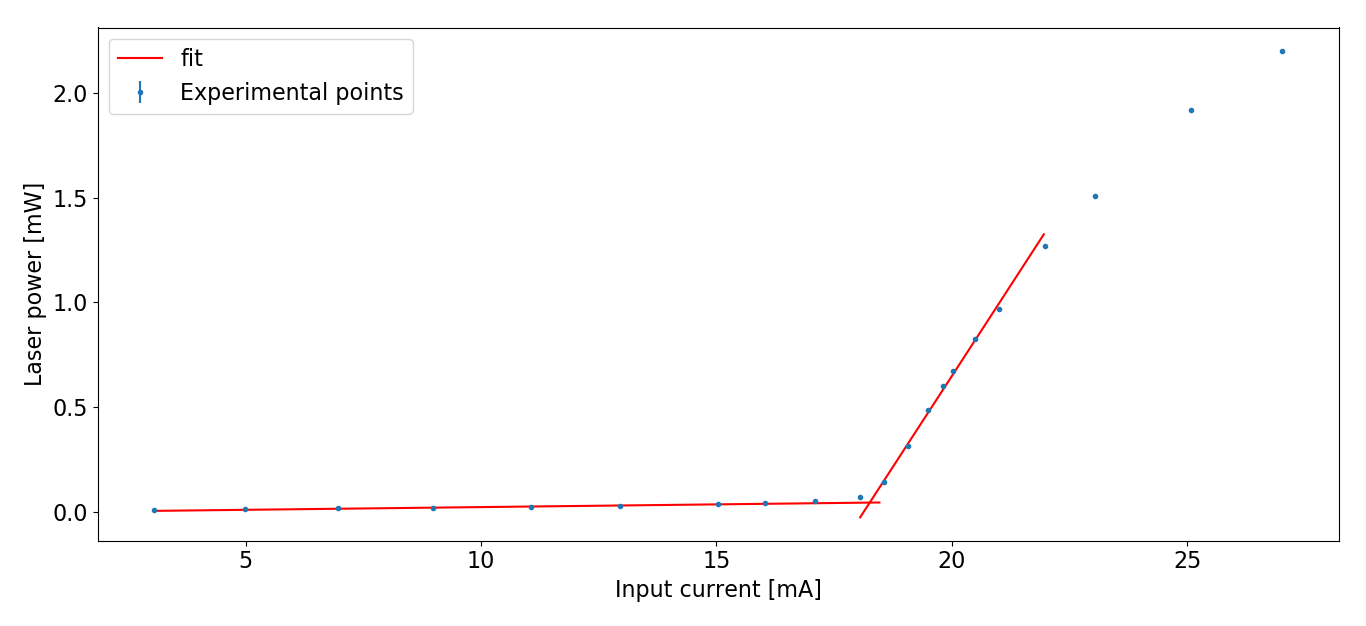
\includegraphics[width=\textwidth]{curvefreerunning.png}
\caption{Characteristic curve of the free running laser diode, errorbars are too small to be seen}\label{curvefreerunning}
\end{figure}
The first task that we performed was to measure the characteristic curve of the free running diode laser. We measured the output power of the laser with a powermeter as a function of the input current. We took 5 seconds of measurement which is 20 samples, and we calculated the mean and the standard deviation of the mean with the built-in functions of the power meter. These data are shown in figure \ref{curvefreerunning}. To determine the lasing threshold we fitted our data with two lines. The first line is fitted on the data before the lasing threshold, the second line is fitted on the other data. Then the lasing threshold is calculated as the interception of these two lines. If we write the left line as $y=a_l + b_lx$, and the right line as $y = a_r +b_r x$, the abscissa of the interception is:
\begin{equation}x_i = \frac{a_l-a_r}{b_r-b_l}.\end{equation}
The error is calculated through propagation on this formula. We found a lasing threshold of $I_l = 18.2\pm 0.4$ mA.
\subsection{Littrow configuration}
\begin{figure}[H]
\centering
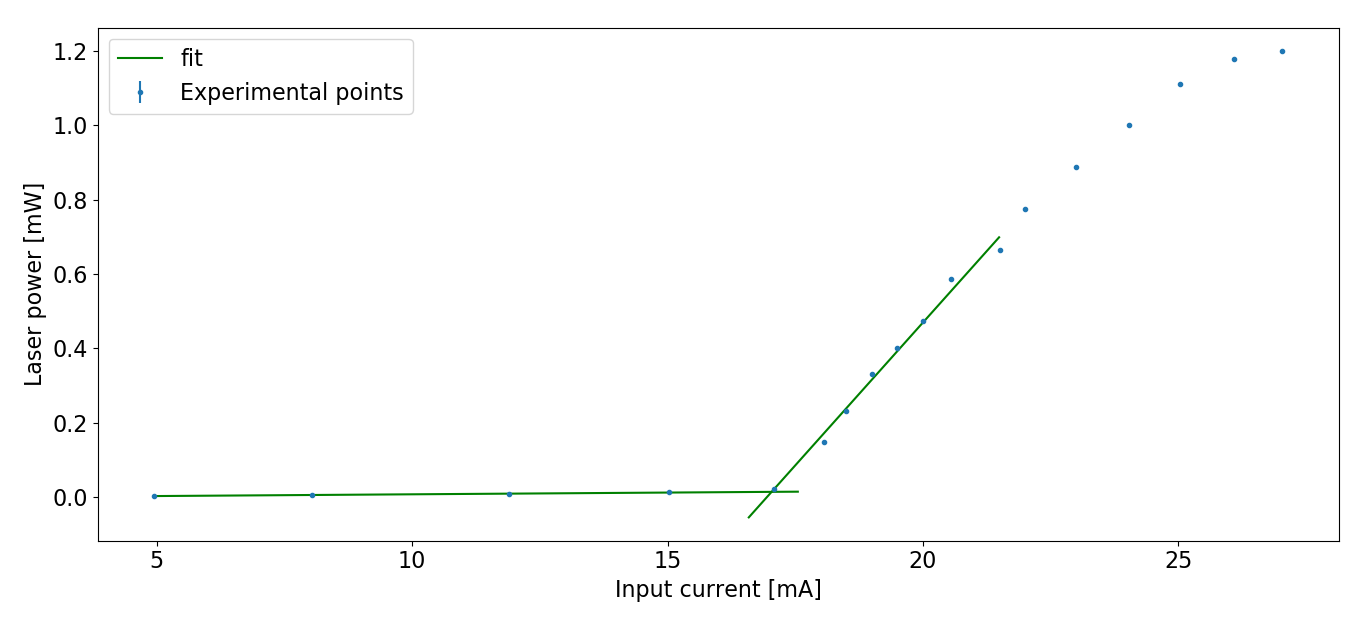
\includegraphics[width=\textwidth]{curvelittrow.png}
\caption{Characteristic curve of laser diode in the Littrow configuration, errorbars are too small to be seen}\label{littrowcurve}
\end{figure}
We built the Littrow configuration as shown in figure \ref{littrow}, then we measured again the characteristic curve with the same method described in the previous section. The acquired data can be seen in figure \ref{littrowcurve}. The lasing threshold is determined with the same procedure as before. We found a lasing threshold of $I_l =17.0 \pm 0.5$ mA. We can notice that this threshold is lower than the threshold of laser without feedback. It is a consequence of the feedback field which change the gain inside of the laser and thus the lasing threshold is reached sooner.\\
In the Littrow configuration we calculated also the wavelength of the laser. This can be done geometrically, the incident angle $\alpha$ can be found with the law of cosines applied on the triangle in figure \ref{littrow} where at the vertices there are the laser, the powermeter and the grating. Angles of the diffracted beams are related via the grating equation \cite{grating}
\begin{equation}\label{grating}m\lambda = d(\sin \alpha + \sin \beta),\end{equation}
where $m$ is the order of diffraction, $\lambda$ the wavelength of the laser, and $\beta$ is the diffraction angle. From this equation we can see that for the zeroth order it must hold $\alpha = -\beta$, which justifies the angles in figure \ref{littrow}. We measured the sides of this triangle with a measuring tape: from the laser to the powermeter $a = 4.5 \pm 0.1$ cm, from the laser to the grating $b = 6.0\pm 0.1$ cm, and from the grating to the powermeter $c = 6.5\pm 0.1$ cm. The error is the resolution of the measuring tape. The law of cosines states that
\begin{equation}a^2 = b^2 + c^2 -2bc\cos(2\alpha).\end{equation}
We can work out $\alpha$ to obtain
\begin{equation}\alpha = \frac{1}{2}\arccos\left(\frac{b^2 + c^2 - a^2}{2bc}\right).\end{equation}
We can now use the grating equation \eqref{grating} on the first diffracted order, keeping in mind that this order is the feedback, so the incident angle $\alpha$ is equal to the diffraction angle:
\begin{equation}\lambda = 2d\sin(\alpha).\end{equation}
Putting together the last two equation we end up with the final formula
\begin{equation}\label{wavelength}\lambda = 2d\sin\left(\frac{1}{2}\arccos\left(\frac{b^2 + c^2 - a^2}{2bc}\right)\right).\end{equation}
With our data we obtained $\lambda = 597\pm15$ nm. The error is calculated through error propagation on equation \eqref{wavelength}. This result is not exactly what we expected from a red laser, but probably the error is underestimated due to the physical difficulty of determining the exact vertices of the triangle. A better approach could have been taken, for example by extending the sides of the triangle to a bigger rectangle triangle and performing the measurements on the latter triangle. The error on the measure is still the same, but the relative error would be much smaller.
\subsection{Littman configuration}
\begin{figure}[H]
\centering
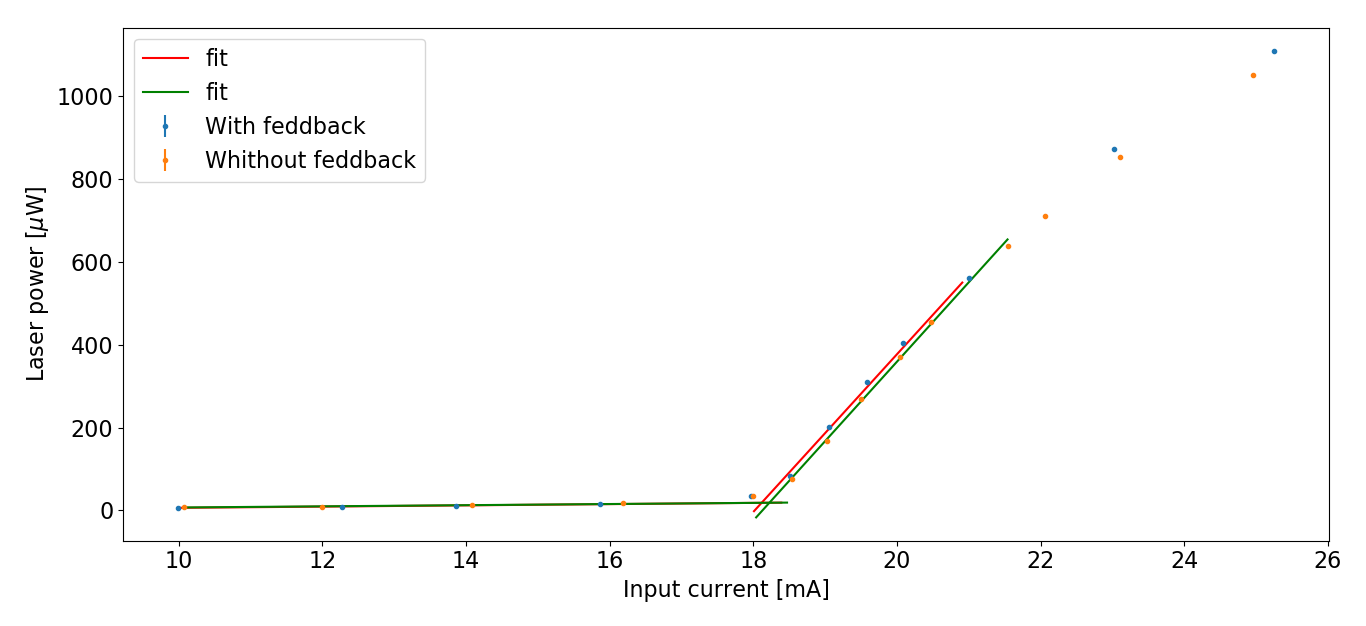
\includegraphics[width=\textwidth]{curvelittman.png}
\caption{Characteristic curve of laser diode in the Littman configuration, errorbars are too small to be seen}\label{littmancurve}
\end{figure}
In this part of the experiment we built the setup in figure \ref{littman}. We measured again the characteristic curve, with and without feedback. The power of the zeroth order is measured with the same powermeter as before and with the same method. In figure \ref{littmancurve} these measurements can be seen. The same analysis of the previous section on the characteristic curve has been done, we found a lasing threshold of $I_l =18.1\pm 0.4$ mA for the measurement with feedback, and $I_l = 18.2 \pm 0.3$ mA without feedback. We can clearly see that the feedback does not play a role in the Littman configuration for the lasing threshold, furthermore in both cases it is higher that the threshold of the laser in the Littrow configuration.\\
Again with geometrical arguments the wavelength can be found. Compared to the Littrow configuration the Littman is more complex, so in the following analysis we will refer to the simplified geometrical figure \ref{geometry}. We measured the following quantities: $a = 8\pm0.1$ cm, $b= 9.5\pm 0.1$ cm, $c = 16.5\pm0.1$ cm, $d = 17.0\pm0.1$ cm, $e = 23.0\pm0.1$ cm, $f = 10.0\pm0.1$ cm, $g = 7.8\pm0.1$ cm, and $h = 209.0\pm0.1$ cm. The goal of the geometric analysis is to find $\lambda$ from the grating equation applied to the first diffracted order
\begin{equation}\lambda = d(\sin\alpha + \sin\beta).\end{equation}
We can use the law of cosine to calculate almost every angle:
\begin{multline}\gamma = \arccos\left(\frac{c^2+e^2-d^2}{2ce}\right) = 47.5\pm0.4\,^\circ \quad  \theta = \arccos\left(\frac{a^2+c^2-b^2}{2ab}\right) = 21.3\pm 1.8\,^\circ \\ \Gamma = \arccos\left(\frac{c^2+d^2-e^2}{2cd}\right)=86.7\pm 0.6\,^\circ.\end{multline}
In order to find $\alpha$ we need $j$ which can be found in the following way
\begin{equation}j^2 = a^2 + d^2 - 2ad\cos(\theta+\Gamma) = 437\pm 10 \, \text{cm}^2,\end{equation}
with this value we can finally determine
\begin{equation}\alpha = \frac{1}{2}\arccos\left(\frac{b^2+e^2-j^2}{2be}\right) = 32.6\pm 0.8\,^\circ.\end{equation}
Now we only need $\beta$ which is $\beta = \gamma -\alpha = 14.9\pm 0.9\,^\circ $. Therefore, with the grating equation we arrive at the wavelength $663.9\pm 0.9$ nm. All the errors are calculated with propagation. This result is more plausible compared to the result obtained in the Littrow configuration.

\begin{figure}[H]
\centering
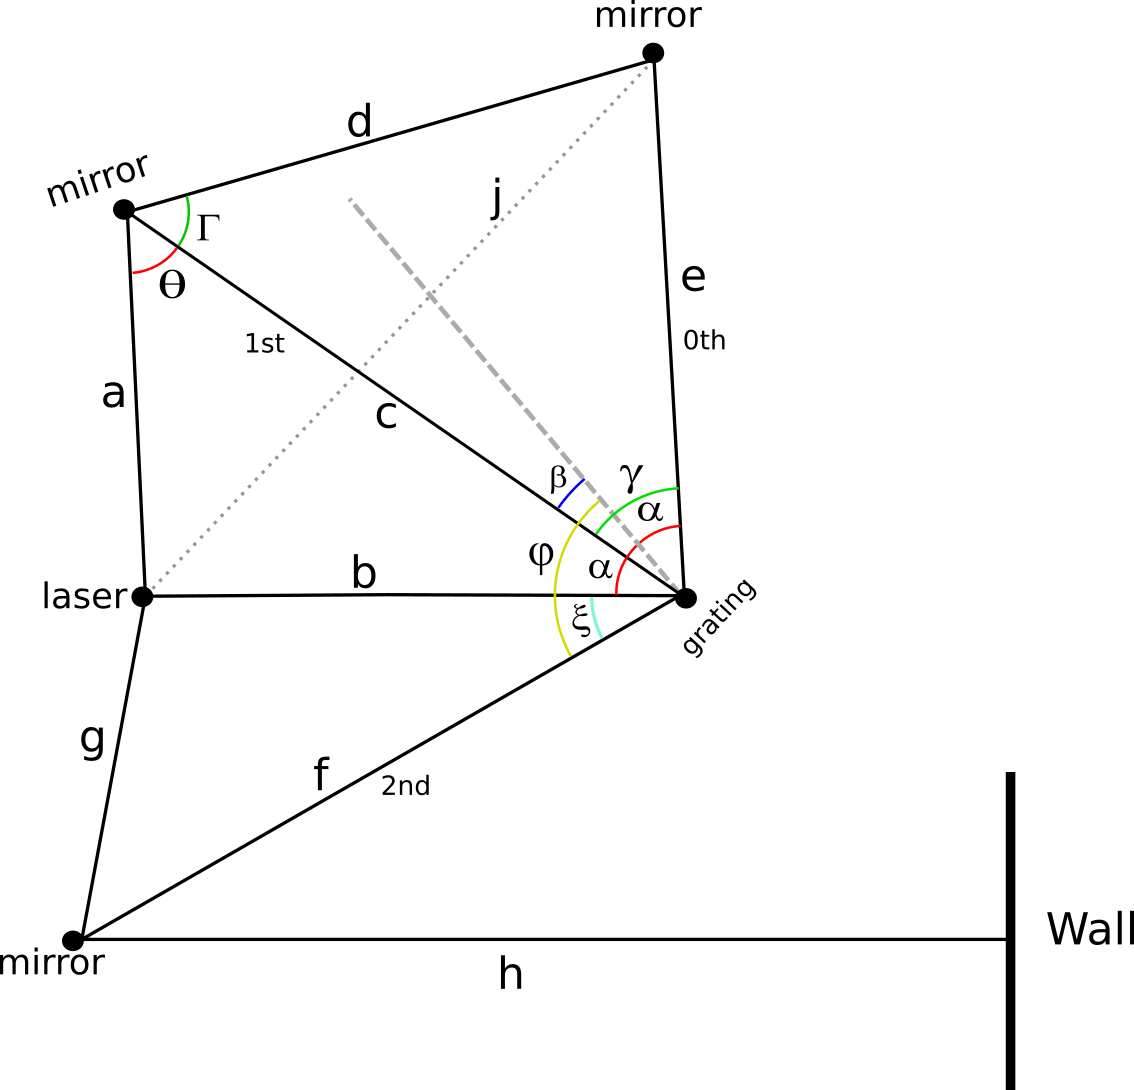
\includegraphics[width=.7\textwidth]{geometry.png}
\caption{Geometry of the Littman configuration, not in scale}\label{geometry}
\end{figure}
\subsection{Laser tunability}
\begin{figure}[H]
\centering
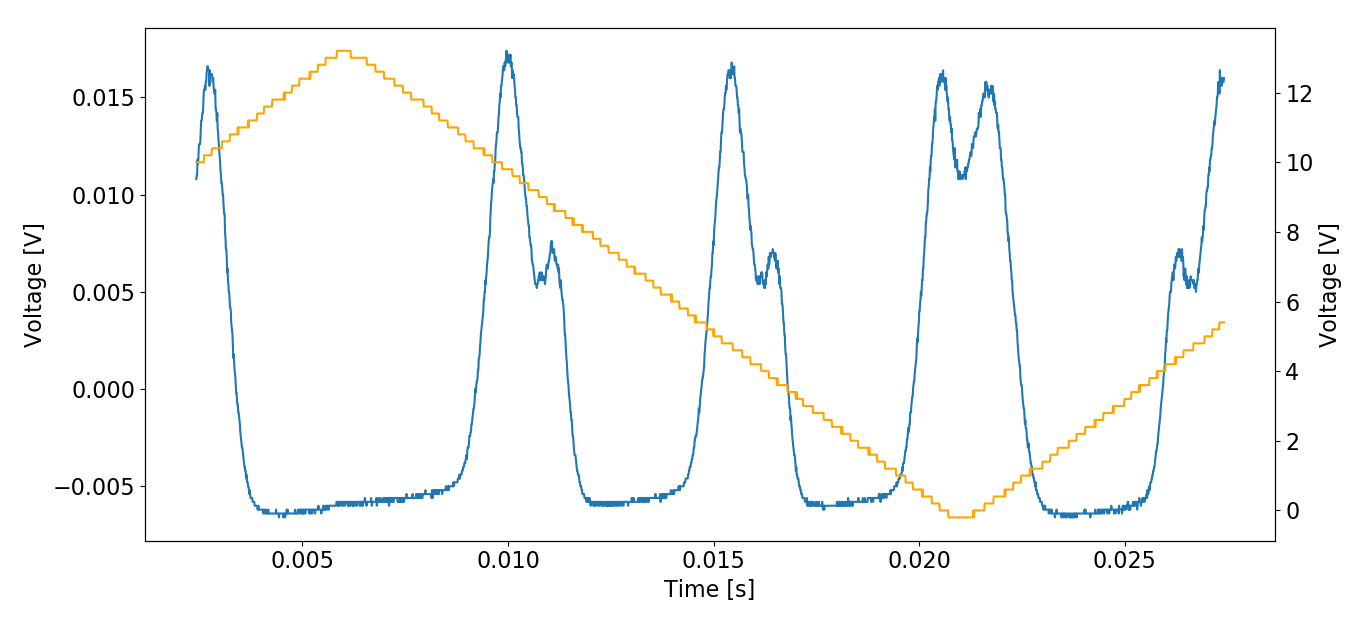
\includegraphics[width=\textwidth]{fabryperot.png}
\caption{Spectrum of the Fabry-Perot and electrical signal of the piezoelectric crystal. Scales are different, the left axis is for the blue data, the right axis is for the orange data}\label{fabryperot}
\end{figure}
In the last part of this experiment we looked at the laser tunability in the Littman configuration. First we marked the spot on the wall where the laser had its maximum intensity, then we proceeded to horizontally dealign the mirror used for the feedback.\\
We acquired the signal of the photodiode and the electric signal from the function generator used to change the distance between the mirrors. This data can be seen in figure \ref{fabryperot}. The photodiode signal is in blue, in fact we can seen the typical peaks. The small peaks on the side are due to the misalignment, while the double peak is due to change in the motion of the mirrors, as can be seen in the signal of the crystal which changes slope. In order to obtain the free spectral range (FSR), we must convert the signal from a time dependence to a frequency one. This can be done by measuring the distance between one peak and its side peak and then comparing this with the frequency change caused by the misalignment. This can be found geometrically by comparing the distance of the previously marked spot and the new maximum after the misalignment on the wall. For the following analysis we will always refer to figure \ref{geometry}. Misaligning the feedback mirror causes a shift $\Delta x$ on the peak on the wall. This is related to a change in the angle $\Delta \varphi$
\begin{equation}\Delta \varphi = \frac{\Delta x}{f+h}.\end{equation}
If we use the grating equation \eqref{grating} where now $\alpha = \varphi$, the change in $\varphi$ is equivalent in a change of wavelength
\begin{equation}\Delta \lambda = \frac{d}{2}\cos(\varphi)\Delta \varphi.\end{equation}
The shift in wavelength can be related easily to a frequency shift $df = c/\lambda^2 d\lambda$, where $c$ is the speed of light, and for the wavelength $\lambda$ we can use the result that we found in the previous section. In conclusion the relation between the shift of the peak on the wall and the shift in frequency is
\begin{equation}\Delta f = \frac{cd}{\lambda^2} \cos(\varphi)\frac{\Delta x}{f+g}.\end{equation}
$\varphi$ can be found geometrically by $\varphi = \alpha + \xi$, where $\xi$ can be calculated with the law of cosine applied to the triangle $bgf$. From our data we obtained $\Delta f = 460.8 \pm 0.8$ GHz, the error has been propagated over all the formulas.\\
This frequency shift has to be compared to the difference in time between a peak and its side peak, this information can be extrapolated from our data with a fit. We isolated the peaks we are interested in, and we fitted a sum of two Lorentz functions with the following form
\begin{equation}f(t) = V_{offset}+\sum_{i=1}^2 A_i \frac{\Gamma_i}{(t-t_{0i})^2 + \Gamma_i^2},\end{equation}
where $t_0$ is the center of the peak, $A_i$ a parameter, and $\Gamma_i$ is the HWHM. This fit can be seen in figure \ref{fit}. The relevant fit parameters are the center of the peaks, which we found to be $t_{0} = 9.999 \pm 0.003$ ms for the higher peak, and $t_0 = 11.130\pm  0.005$ ms for the side peak. Now we can convert the time in frequency by multiplying the time for $\Delta f/\Delta t$, where $\Delta t$ is the distance between the peak and its side peak that we have just found.\\
We can finally calculate the free spectral range, we can fit the other peak in figure \ref{fabryperot} and measuring the distance in frequency between the peak we just fitted and the other one. This last fit is shown in figure \ref{fit2}, where the higher peak has a center of $t_0 = 15.430\pm 0.003$ ms. Finally we obtained for the free spectral range $\text{FSR}  = 2214.6\pm 11.7$ GHz, the error is propagated from all the previous errors.
\begin{figure}[H]
\centering
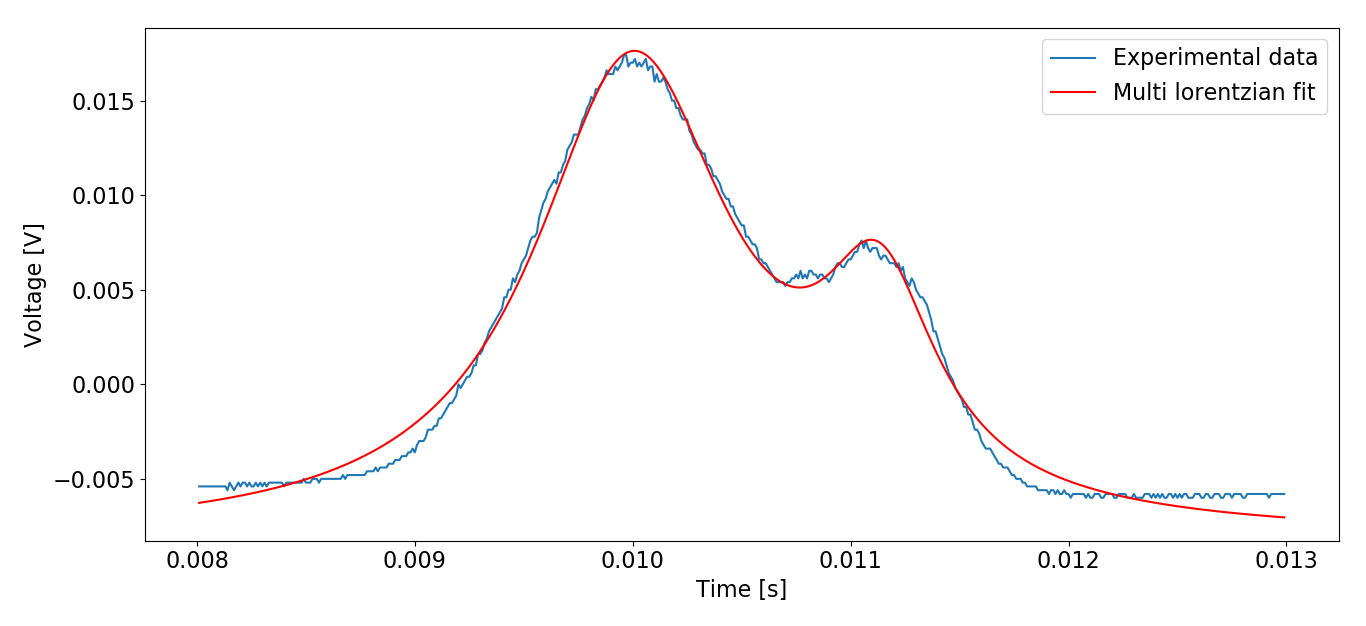
\includegraphics[width=\textwidth]{fit.png}
\caption{Multi Lorentzian fit, we assumed an error on the data given by the resolution of the oscilloscope, i.e. the full scale divided by 8 bit of resolution that is $2^8$}\label{fit}
\end{figure}
\begin{figure}[H]
\centering
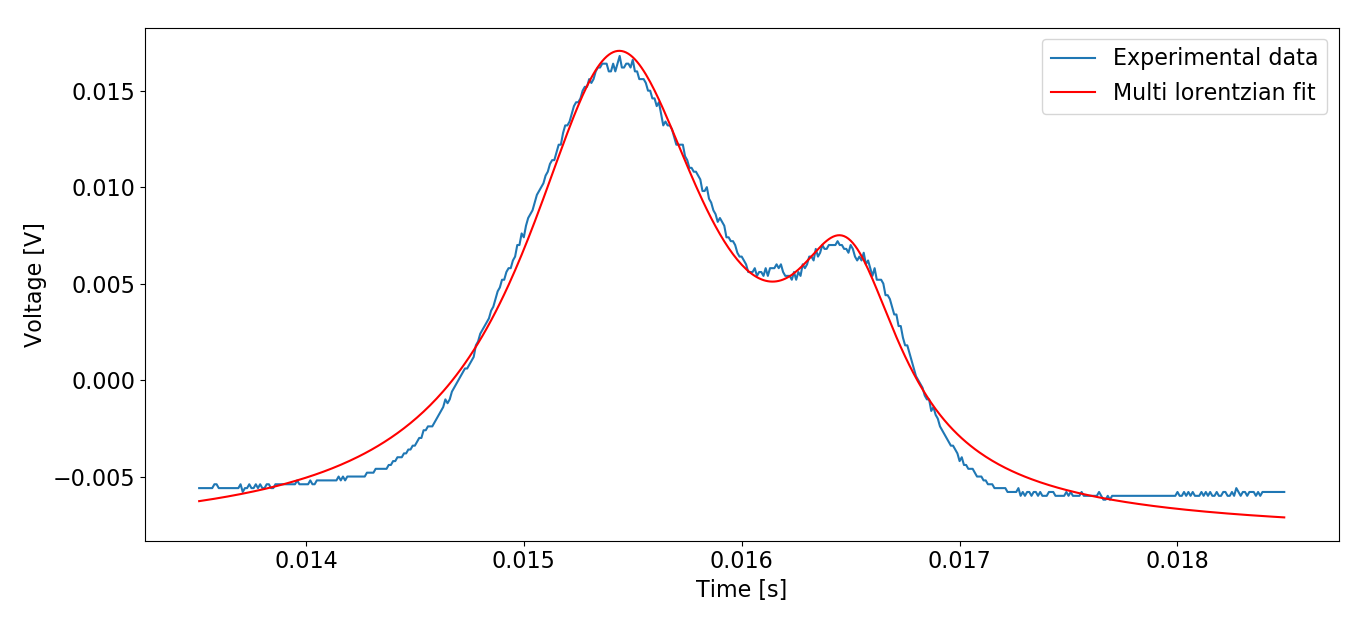
\includegraphics[width=\textwidth]{fit2.png}
\caption{Multi Lorentzian fit, we assumed an error on the data given by the resolution of the oscilloscope, i.e. the full scale divided by 8 bit of resolution that is $2^8$}\label{fit2}
\end{figure}
\section{Discussion and conclusion}
In this work we analyzed the impact of optical feedback on a diode laser. We explored two different configuration for the external cavity: Littrow, and Littman. First for every configuration and for the free-running laser we analyzed the characteristic curve with a particular focus on the lasing threshold. In the Littrow configuration this threshold was lower compared to the free-running laser and the Littman configuration which all showed a very similar lasing threshold, this is a consequence of the feedback which increase the gain inside the laser, and thus the lasing threshold is reached sooner. Exploiting the geometry of the configurations we found two values for the wavelength of the laser which are not too similar, however the result of 663 nm in the Littman configuration looks more reasonable. For the last part we found a free spectral range of around 2000 GHz, which is higher then expected, probably the error has been underestimated.
\begin{thebibliography}{99}
\bibitem{skriptum}
\textsc{M. Jag,T. Northup}, \textit{Exercise FP2-09: Diode Laser With Optical Feedback}, Fortgeschrittenenpraktikum 2.

\bibitem{tunablelaser}
\textsc{F.J. Duarte}, \textit{Tunable Lasers Handbook} A volume in Optics and Photonics (Academic, New York, 1995). 

 \bibitem{lasertunability}
 \textsc{Carl E. Wieman}, \textit{Using diode lasers for atomic physics}, Review of Scientific Instruments 62,1 (1991).
 
\bibitem{lasermodulation}
    \textsc{K. Petermann}, \textit{Laser Diode Modulation and Noise}, Advances in Optoelectronics (ADOP).

\bibitem{grating}
\textsc{Palmer Christopher}, \textit{Diffraction Grating Handbook} (7th edition) Richardson Gratings (2014). 

\bibitem{linewidthformula}
\textsc{A. L. Schawlow and C. H. Townes}, \textit{Infrared and optical masers}, Phys. Rev. 112 (6), 1940 (1958)
\bibitem{feedback}
\textsc{J. Osmundsen,N. Gade}, \textit{Influence of optical feedback on laser frequency spectrum and threshold conditions}, IEEE Journal of Quantum Electronics 19,3 (1983).

\end{thebibliography}
\end{document}
